%% The commands defining this class, which inherits from the article class, are found in project.cls
%% this is a comment, btw
\documentclass{project}

%% The first part of the file, before \begin{document}, is the preamble and does not directly create output

%% The title author and date are defined outside the document scope.
\title{Example project}
\author{E. Person}
\date{\today}

%% Tell it where to look for citations (note this is a biblatex package command)
\addbibresource{example.bib}

%% Everything after this is part of the document
\begin{document}

%% The project class uses the "titling" package to make a title page with abstract that can use the convenient \maketitle command
%% Turning off pageanchors for the title page helps hyperref avoid a double page label, leading to a warning. 
\hypersetup{pageanchor=false}
\begin{titlingpage}
\maketitle

%% The titling page will format the abstract, we just have to write it in between the begin and end commands.
\begin{abstract}
In this note, the results of the example project for the computation of numerical integrals are discussed. Using two example potentials, the differential cross sections in the first Born approximation are computed using the trapezoid rule. This is compared with the results of a more sophisticated integration and with the exact solutions. This note also serves as an introduction to writing articles in \LaTeX.
\end{abstract}

\end{titlingpage}
\hypersetup{pageanchor=true}

%% After this point the main document's body begins.
%% For complex documents, it's helpful to write section in their own files and add them with \input


%%%%%%%%%%%%%%%%%%%%%%%%%%%%%%%%%%%%%%%%%%%%%%%%%%%%%%%%%%%%%%%%%%%%%%%%%%%%%%%%%%
%% I like obvious comment marks between bits, especially in long documents
%%%%%%%%%%%%%%%%%%%%%%%%%%%%%%%%%%%%%%%%%%%%%%%%%%%%%%%%%%%%%%%%%%%%%%%%%%%%%%%%%%
\section{Introduction}

The cross section for scattering of non-relativistic quantum particles from weak central potentials can be approximated
%% Cite an entry from the .bib . Note a line break in the tex file does not break the paragraph! 
%% Also, the ~ is a non-breaking space to ensure the citation stays on the same line in the document
using the Born approximation~\cite{Born1926}. 
%% The ket notation, vector symbols, and derivative command come from the "physics" package loaded by project.cls
The first order approximation involves the matrix element of the potential between initial and final momentum states $\ket{\va{p}_i}$ and $\ket{\va{p}_f}$.
The differential scattering cross section is obtained from the integral:
\begin{equation} %% Nice display math with equation numbering
      \dv{\sigma}{\Omega} = \abs{ \frac{m}{2\pi\hbar^2} \int e^{-i\vb{q}\cdot \vb{r}'} V(\vb{r}') \dd[3]{r'} }^2,
\end{equation}
where the momentum transfer $\hbar\va{q} = \va{p}_f-\va{p}_i$, $\sigma$ is the cross section, $\Omega$ is the solid angle, and $m$ is the mass of the incoming particle.
For spherically symmetric potentials, the differential cross section depends only on the angle with respect to the incoming direction, $\theta$, and the integral reduces to one over only the radial coordinate: 
\begin{equation}
\dv{\sigma}{\Omega} =  \abs{\frac{-2m}{\hbar^2} \int_0^\infty \frac{\sin qr'}{q} V(r') r' \dd{r'}}^2,
\end{equation}
where $q = 2k \sin(\theta/2)= 2p \sin(\theta/2)/\hbar$.

%%A line of whitespace causes a paragraph break
While for some functional forms it is possible to analytically integrate to find the differential cross section, this is not possible in general. Numerical integration is thus a useful tool to employ. 
In this note, I will compare the solutions obtained from numerical integration with the exact solutions for two example potentials: the square well potential and the Yukawa potential~\cite{Yukawa:1935xg},
\begin{align} %% Align lines up the '&' symbols (they don't appear in the displayed math). \\ is a line break
  %% cases formats the curly braces used to describe a piecewise function
  V_{\text{square}}(r) &= \begin{cases} V_0 & r < a \\ 0 & r > a \end{cases}, \\
  V_{\text{Yukawa}}(r) &=  \frac{V_0 a e^{-r/a}}{r},
\end{align}
where $V_0$ gives the overall strength of the potential and $a$ its length scale. When computing numerical integrals, it is helpful to reduce the problem to one that is unitless. To this end, I define the incoming wave number of the scattered particle in terms of $a$ by using $ka = p_i a/\hbar$, ensure all potentials are given as $V_0$ times a unitless function, and use $r/a$ as the variable of integration. We have, then, that the number obtained for the cross section is in units of $a^2$ multiplied by a ratio between the kinetic and potential energy scales:
\begin{equation}
  \sigma_0 = \qty(\frac{2ma^2V_0}{\hbar^2})^2 a^2.
\end{equation}

The analytic solutions for the Born approximation applied to the Yukawa and square well potentials are respectively
\begin{align}
  \dv{\sigma}{\Omega} &= \frac{\sigma_0}{ ( 1 + q^2a^2 )^2 }  \\
  \intertext{and}
  \dv{\sigma}{\Omega} &=\sigma_0 \frac{1}{\qty(qa)^4}  \qty[ \frac{\sin(qa)}{qa} - \cos(qa) ].
\end{align}



%%%%%%%%%%%%%%%%%%%%%%%%%%%%%%%%%%%%%%%%%%%%%%%%%%%%%%%%%%%%%%%%%%%%%%%%%%%%%%%%%%
%%%%%%%%%%%%%%%%%%%%%%%%%%%%%%%%%%%%%%%%%%%%%%%%%%%%%%%%%%%%%%%%%%%%%%%%%%%%%%%%%%
\section{Implementation}

To explore the effects parameters of the numerical integration have on its accuracy, I compare the exact solutions with both a simple integral approximation, as well as the more sophisticated SciPy~\cite{2020SciPy-NMeth} \texttt{quad} method from the \texttt{integrate} package. The potentials and their analytical cross sections are implemented as custom python functions. An instance of an integrator class can be created for any potential function that can return two types of numerical integrals:
\begin{enumerate}
\item A simple application of the trapezoid rule to compute the integral. The range of the integral in terms of $r/a$ and the number of points at which to evaluate the integrand can be configured using properties of the integrator class.
\item The result of the integral using the SciPy \texttt{quad} method with its default parameters. This uses the FORTRAN QUADPACK library, which uses Gauss–Kronrod quadrature to compute the integral. The range of the integral is set as for the trapezoid calculation.
\end{enumerate}
In both cases, the user must specify the parameters $\theta$ and $ka$ of interest. I also use the python \texttt{timeit} module to get a sense of the processing time needed for each algorithm.

%%%%%%%%%%%%%%%%%%%%%%%%%%%%%%%%%%%%%%%%%%%%%%%%%%%%%%%%%%%%%%%%%%%%%%%%%%%%%%%%%%
%%%%%%%%%%%%%%%%%%%%%%%%%%%%%%%%%%%%%%%%%%%%%%%%%%%%%%%%%%%%%%%%%%%%%%%%%%%%%%%%%%
\section{Results}

I compute the differential cross sections for the Yukawa and square well potentials for the values of incoming momentum $ka=1$ and $ka=10$ respectively. A generic feature of solutions to the Born approximation is that at order one the shape of the cross section is changing rapidly from a roughly uniform distribution at low momentum to a sharp peak near zero at high momentum. I use 100 values of $\theta$ from 0 to $\pi$.

The result for the Yukawa potential is shown in \cref{fig:yukawa}. %% I love cleveref's cref because you don't have to write "Fig.~" or "Figure~" yourself and can even change between them after the fact with one preamble command!
For this potential, even a relatively small number of points achieves a low value for the relative error. All configurations of the integrator are correct to better than 1\%. However, there is a clear limitation for a limited integration range, even though the potential decays exponentially. Using only up to $r/a=10$ results in a relative error of 0.1\% at small $\theta$ that appears as a ``wiggle''.
This error does not come from numerical precision per se; it will remain even if a more sophisticated integral algorithm is used if its integration range is set the same. Increasing the integration range, but using a similar distance between points results in a comparable error, but removes the range source of error. Using 10000 points results in an error on the order of $10^{-4}$. The \texttt{quad} method improves the error, but comes at a cost in processing time. The trapezoid rule calculation with 1000 points takes about \SI{3e-3}{\second} per call, and scales linearly to \SI{0.03}{\second} at 10000 points. The \texttt{quad} algorithm takes about four times that at \SI{0.14}{\second} per call.

\begin{figure}[tbp] %%Tell figure to preferentially place at the top or bottom of the page, or on a page of only figures
  \begin{center}
  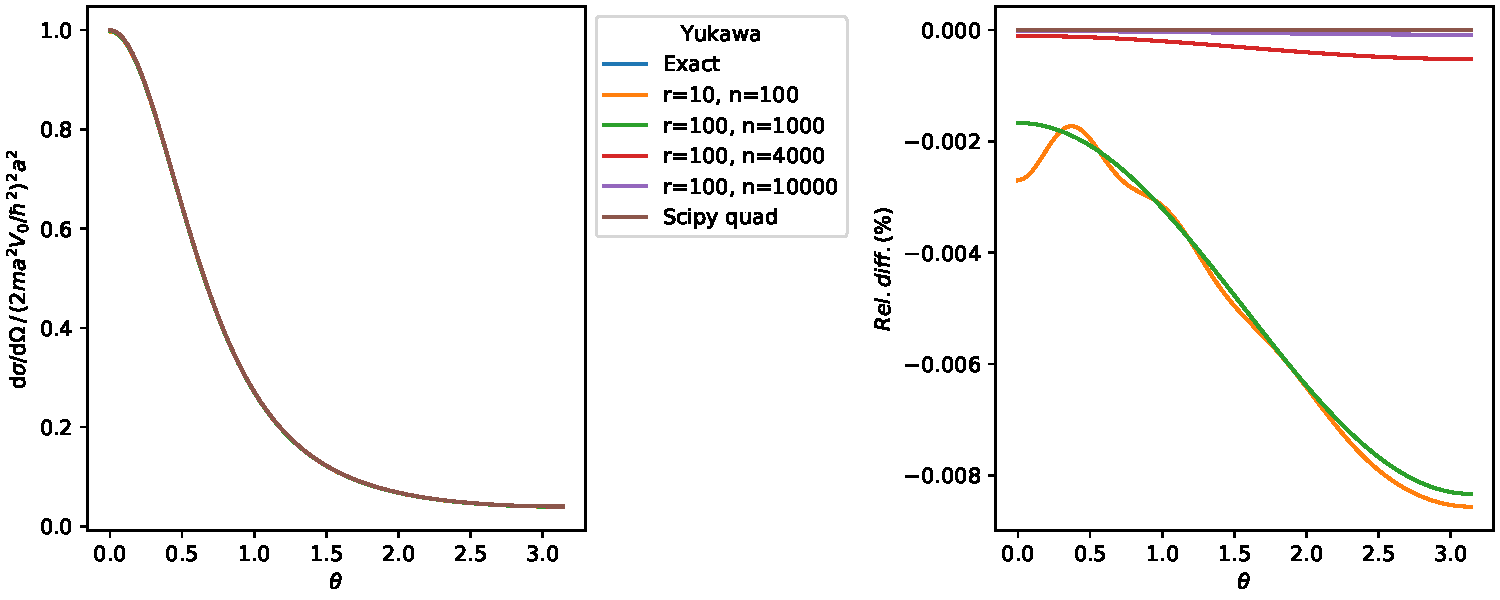
\includegraphics[width=\textwidth]{fig/example/yukawa_born_xs}
  \caption{Results for the Yukawa potential's differential cross section from $\theta=0$ to $\pi$: (left) value in terms of natural units and (right) the relative difference between the exact and numerical solutions. Different integration ranges and numbers of points for the trapezoid rule setup are compared with the result from SciPy \texttt{quad}.\label{fig:yukawa}}
  \end{center}
\end{figure}

The result for the square well potential, shown in \cref{fig:sqwell}, shows some other features related to the fact that the exact solution has zeroes for certain values of $\theta$. Depending on the number of $\theta$ points considered, the numerical value will become very small, but I don't expect to literally reproduce the zero. These small cross sections, however, tend to come with increased relative errors. While the integration range can be small since the integrand is identically zero past $r/a=1$, using only a few hundred points results in relative errors of up to 2\% near the zeroes. This improves greatly with a larger number of points. As for timing, the trapezoid rule calculation is comparable to the Yukawa case, as it scales essentially with the number of points used. The \texttt{quad} method, by contrast, runs approximately twice as fast.

\begin{figure}[tbp]
  %% The main thing about figures is they are *floating*, not at the spot where typed. The typesetting algorithm places them automatically. It will try to get close to where it was entered, following configurable rules about how much of each page can be figures, etc. The options [tbp] request top (t) or bottom (b)  of a page, or allow the figure to appear on a page with only figures and no text (p)
  \begin{center}
  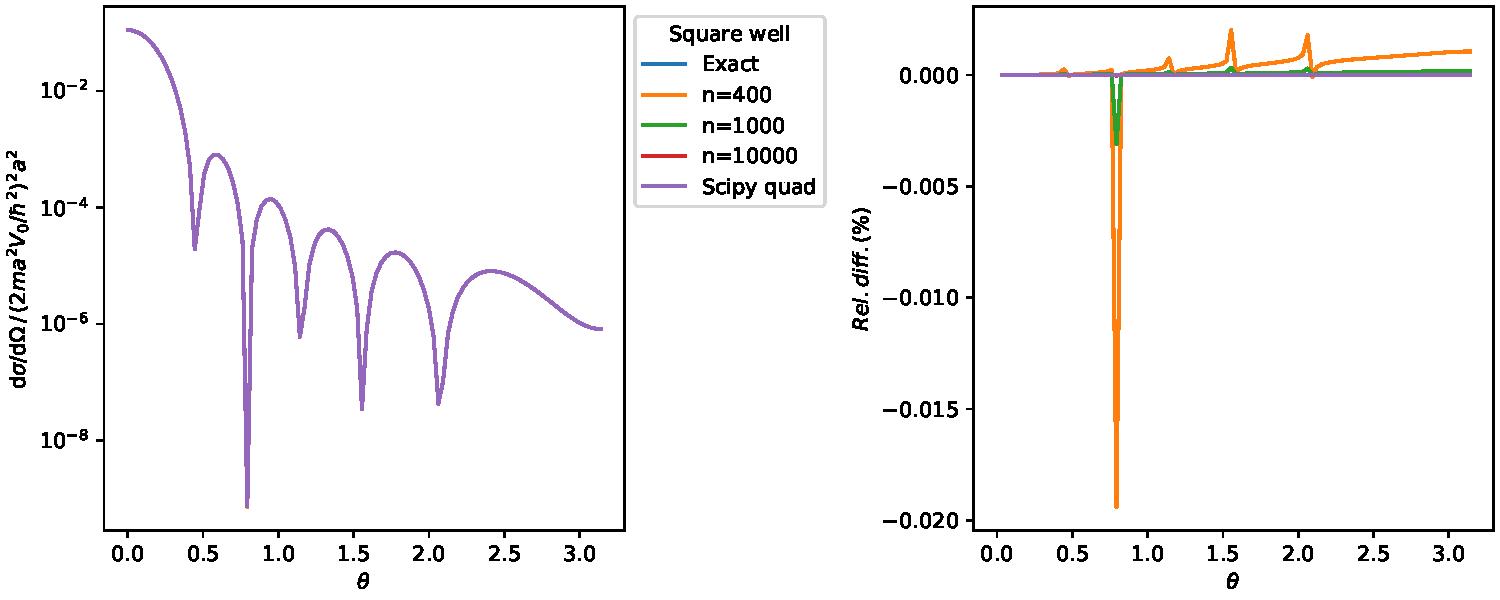
\includegraphics[width=\textwidth]{fig/example/sqwell_born_xs.pdf}
  \caption{Results for the square well potential's differential cross section from $\theta=0$ to $\pi$: (left) value in terms of natural units and (right) the relative difference between the exact and numerical solutions. Different integration ranges and numbers of points for the trapezoid rule setup are compared with the result from SciPy \texttt{quad}.\label{fig:sqwell}}
  \end{center}
\end{figure}

\section{Conclusion}

This study demonstrates a few basic considerations that one has when deciding on a method of numerical computation to employ. Simple algorithms are straightforward to implement and can run very fast. Depending on the tolerance for error needed, they may meet one's needs. They are also more portable, since they do not rely on external dependencies. Established algorithms do, though, bring the advantage of being well tested with a smaller chance of bugs.

%%%%%%%%%%%%%%%%%%%%%%%%%%%%%%%%%%%%%%%%%%%%%%%%%%%%%%%%%%%%%%%%%%%%%%%%%%%%%%%%%%
%% Tell biblatex to add the bibliography entries here
%%%%%%%%%%%%%%%%%%%%%%%%%%%%%%%%%%%%%%%%%%%%%%%%%%%%%%%%%%%%%%%%%%%%%%%%%%%%%%%%%%
\printbibliography

\end{document}
